\documentclass[namedreferences]{solarphysics}
%
% spr-sola-addons available options:
%  hyperref      -- loads hyperref.sty with options (pdfborder={0 0 0 },urlcolor=blue,breaklinks)
%  natbib        -- For citations: redefine \cite commands (loads natbib.sty)
%  solaenum      -- makes enumerated list with italics-roman numerals and a single right-bracket
%  solaromanenum -- makes enumerated list with roman numerals and a single right-bracket
%  linksfromyear -- puts a link on a year citation (hyperref must be loaded)
%  optionalrh    -- for optional running title/author
%
\usepackage[optionalrh,solaromanenum,natbib]{spr-sola-addons}
\usepackage{graphicx}
\usepackage{hyperref}
\usepackage{amssymb}
\usepackage{color}
\usepackage{breakurl}
\usepackage{savesym}
\savesymbol{iint}
\savesymbol{iiint}

\usepackage{amsthm, amsmath}
\def\UrlFont{\sf}
\usepackage{tikz}
\usepackage{subfig}
\usetikzlibrary{fadings}
\numberwithin{equation}{section}

\usepackage{geometry}
\usepackage{pdflscape}

\usepackage{multirow}

\usepackage{booktabs}

% Definitions for the journal names
\newcommand{\adv}{    {\it Adv. Space Res.}} 
\newcommand{\annG}{   {\it Ann. Geophys.}} 
\newcommand{\aap}{    {\it Astron. Astrophys.}}
\newcommand{\aaps}{   {\it Astron. Astrophys. Suppl.}}
\newcommand{\aapr}{   {\it Astron. Astrophys. Rev.}}
\newcommand{\ag}{     {\it Ann. Geophys.}}
\newcommand{\aj}{     {\it Astron. J.}} 
\newcommand{\apj}{    {\it Astrophys. J.}}
\newcommand{\apjl}{   {\it Astrophys. J. Lett.}}
\newcommand{\apss}{   {\it Astrophys. Space Sci.}} 
\newcommand{\cjaa}{   {\it Chin. J. Astron. Astrophys.}} 
\newcommand{\gafd}{   {\it Geophys. Astrophys. Fluid Dyn.}}
\newcommand{\grl}{    {\it Geophys. Res. Lett.}}
\newcommand{\ijga}{   {\it Int. J. Geomagn. Aeron.}}
\newcommand{\jastp}{  {\it J. Atmos. Solar-Terr. Phys.}} 
\newcommand{\jgr}{    {\it J. Geophys. Res.}}
\newcommand{\lrsp}{Living Rev. Solar Phys.}
\newcommand{\mnras}{  {\it Mon. Not. Roy. Astron. Soc.}}
\newcommand{\nat}{    {\it Nature}}
\newcommand{\pasp}{   {\it Pub. Astron. Soc. Pac.}}
\newcommand{\pasj}{   {\it Pub. Astron. Soc. Japan}}
\newcommand{\pre}{    {\it Phys. Rev. E}}
\newcommand{\solphys}{{\it Solar Phys.}}
\newcommand{\sovast}{ {\it Soviet  Astron.}} 
\newcommand{\ssr}{    {\it Space Sci. Rev.}}


% the following is to alter tikz settings to improve springs figure.
\usetikzlibrary{decorations.pathmorphing,calc,patterns}
\makeatletter
\def\pgfdecorationspringstraightlinelength{0.5cm}
\def\pgfdecorationspringnumberofelement{8}
\def\pgfdecorationspringnaturallength{5cm}
\pgfkeys{%
  /pgf/decoration/.cd,
  spring straight line length/.code={%
    \pgfmathsetlengthmacro\pgfdecorationspringstraightlinelength{#1}},
  spring natural length/.code={%
    \pgfmathsetlengthmacro\pgfdecorationspringnaturallength{#1}},
  spring number of element/.store in=\pgfdecorationspringnumberofelement
}

\pgfdeclaredecoration{coil spring}{straight line}{%
  \state{straight line}[%
    persistent precomputation = {%
      % Compute the effective length of the spring (without the length
      % of the two straight lines): \pgfdecorationspringeffectivelength
      \pgfmathsetlengthmacro{\pgfdecorationspringeffectivelength}%
        {\pgfdecoratedpathlength-2*\pgfdecorationspringstraightlinelength}
      % Compute the effective length of one coil pattern:
      % \pgfdecorationspringeffectivelengthofonecoil
      \pgfmathsetlengthmacro{\pgfdecorationspringeffectivelengthofonecoil}%
        {\pgfdecorationspringeffectivelength/\pgfdecorationspringnumberofelement}
    },
    width = \pgfdecorationspringstraightlinelength,
    next state = draw spring]{%
      \pgfpathlineto{%
        \pgfqpoint{%
          \pgfdecorationspringstraightlinelength}{0pt}}
  }
  \state{draw spring}%
    [width=\pgfdecorationspringeffectivelengthofonecoil,
     repeat state=\pgfdecorationspringnumberofelement-1,next state=final]{%
       \pgfpathcurveto
         {\pgfpoint@onspringcoil{0    }{ 0.555}{1}}
         {\pgfpoint@onspringcoil{0.445}{ 1    }{2}}
         {\pgfpoint@onspringcoil{1    }{ 1    }{3}}
       \pgfpathcurveto
         {\pgfpoint@onspringcoil{1.555}{ 1    }{4}}
         {\pgfpoint@onspringcoil{2    }{ 0.555}{5}}
         {\pgfpoint@onspringcoil{2    }{ 0    }{6}}
       \pgfpathcurveto
         {\pgfpoint@onspringcoil{2    }{-0.555}{7}}
         {\pgfpoint@onspringcoil{1.555}{-1    }{8}}
         {\pgfpoint@onspringcoil{1    }{-1    }{9}}
       \pgfpathcurveto
         {\pgfpoint@onspringcoil{0.445}{-1    }{10}}
         {\pgfpoint@onspringcoil{0    }{-0.555}{11}}
         {\pgfpoint@onspringcoil{0    }{ 0    }{12}}
  }
  \state{final}{%
    \pgfpathlineto{\pgfpointdecoratedpathlast}
  }
}

\def\pgfpoint@onspringcoil#1#2#3{%
  \pgf@x=#1\pgfdecorationsegmentamplitude%
  \pgf@x=.5\pgf@x%
  \pgf@y=#2\pgfdecorationsegmentamplitude%
  \pgfmathparse{0.083333333333*\pgfdecorationspringeffectivelengthofonecoil}%
  \pgf@xa=\pgfmathresult pt
  \advance\pgf@x by#3\pgf@xa%
}

\makeatother

\tikzset{%
  Spring/.style = {%
    decoration = {%
      coil spring,
      spring straight line length = 0.2cm,
      % To be added
      spring natural length = #1,
      spring number of element = 4,
      amplitude=2mm},
    decorate,
    very thick},
  Spring/.default = {4cm}}
%%%%%%%%%%%%%%%%%%%%%%%%%%%%%%%%%%%%%%%%%%%%%%%%%%%%%%%%%%%%%%%%%%
\begin{document}

\begin{article}

\begin{opening}

\title{Solar Magneto-seismology with Magneto-acoustic Surface Waves in Asymmetric Magnetic Slabs Waveguides}

\author[addressref={UoS},email={}]{\inits{M.}\fnm{Matthew }\lnm{Allcock}\orcid{0000-0002-0771-743X}}

\author[addressref={UoS},corref,email={robertus@sheffield.ac.uk}]{\inits{R.}\fnm{Robert }\lnm{Erd\'{e}lyi}\orcid{0000-0003-3439-4127}}

%%%%%%%%%%%%%%%%%%%%%%%%%%%%%%%%%%%%%%%%%%%%%%%%%%%
%% Runningheads
%
\runningauthor{M. Allcock, R. Erd\'{e}lyi}
\runningtitle{Solar Magneto-Seismology with Asymmetric Slab Waveguides}
%%%%%%%%%%%%%%%%%%%%%%%%%%%%%%%%%%%%%%%%%%%%%%%%%%%
%%Affilations 

\address[id={UoS}]{Solar Physics and Space Plasma Research Centre, School of Mathematics and Statistics, University of Sheffield, Hicks Building, Hounsfield Road, Sheffield, S3 7RH, UK.}


%%%%%%%%%%%%%%%%%%%%%%%%%%%%%%%%%%%%%%%%%%%%%%%%%%%
% Abstract 
\begin{abstract}
Solar magneto-seismology is a method used to approximate plasma parameters that are traditionally difficult to measure using observations of magneto-hydrodynamic waves. A magnetic slab can act as waveguide for magneto-acoustic waves that approximates magnetic structures in the Solar atmosphere. Asymmetry of the slab caused by different plasma parameters in each external region distorts both the eigenfrequencies and eigenfunctions of the system, that is both the temporal and spatial profiles of the waves that propagate along the slab. We present two novel diagnostic tools for solar magneto-seismology that use this distortion to estimate the slab magnetic field strength using the spatial distribution of  magneto-acoustic surface waves: the \emph{amplitude ratio} and the \emph{minimum perturbation shift} methods. These methods can be used to approximate background parameters that are traditionally difficult to measure in inhomogeneous structures such as elongated magnetic bright points, prominences, and the locally slab-like magnetic structures above sunspot light bridges known as light walls, that may be locally approximated as slabs.
\end{abstract}

%%%%%%%%%%%%%%%%%%%%%%%%%%%%%%%%%%%%%%%%%%%%%%%%%%%
%% Keywords
\keywords{Coronal Seismology; Magnetic fields, Photosphere; Waves, Magnetohydrodynamic; Waves, Modes.}
\end{opening}
%-------------------------------------------------
%%%%%%%%%%%%%%%%%%%%%%%%%%%%%%%%%%%%%%%%%%%%%%%%%%%

\section{Introduction}
The emerging field of solar magneto-seismology (SMS) has become a crucial tool in developing our understanding of solar structures. By comparing observational measurements of magnetohydrodynamic (MHD) waves to the wave solutions in inhomogeneous plasma models, we can make approximations of traditionally difficult-to-measure parameters such as the magnetic field strength and heat transport coefficient \citep{nak_etal05,arr12,dem_etal12}. This in turn equips us with more realistic parameters for numerical simulations and give us a better understanding of conditions that lead to, for example instability, magnetic reconnection, and heating.

SMS techniques can be categorised as either temporal or spatial seismology. By temporal seismology we refer to methods that estimate a plasma parameter by using the observed frequency, or equivalently the period, of waves. By spatial seismology we refer to methods that estimate a plasma parameter by comparing the observed spatial and/or temporal wave power distribution with the eigenfunctions from a theoretical model.

Several temporal seisology methods have been employed successfully. \cite{ros70} first suggested that the frequency of oscillations, observed through the fluctuation of synchrotron radiation due to the presence of MHD waves, could be used to diagnose background parameters. Further theoretical development has led to more sophisticated temporal methods including local coronal magnetic field strength estimates using standing kink modes in coronal loops by \cite{nak_etal01}, and using slow sausage and kink modes by \cite{erd_etal08}. The ratio of periods of the fundamental and the first harmonic standing kink mode and its dependence on density stratification has also been well studied \citep{ban_etal07,erd_etal14}.

Spatial seismology techniques have more recently started demonstrating their efficacy in estimating solar parameters. \cite{uch70} estimated the coronal magnetic structure by comparing Moreton wave observations with the theoretical influence that the coronal magnetic field has on the shape of the Moreton wavefront. More recent eigenfunction methods include utilising the anti-node shift of standing modes in a magnetic flux tube to diagnose its inhomogeneous density stratification \citep{ver_etal07,erd_etal14}.

In the present work, we derive two novel analytical tools for spatial seismology that use an asymmetric slab waveguide to approximate background parameters. This has applications to solar atmospheric structures that are locally slab-like which have been observed to guide MHD oscillations, such as elongated magnetic bright points, prominences, and the locally slab-like magnetic structures above sunspot light bridges known as light walls \citep{arr_etal12,yan_etal17,zha_etal17}.

This is an application of the linear wave analysis of asymmetric magnetic slabs completed by \cite{all_etal17}. A magnetic slab, with non-magnetic, but asymmetric density and temperatures outside the slab has eigenmodes which can be described as either quasi-sausage or quasi-kink. For quasi-sausage (quasi-kink) modes, the oscillations on each slab interface are in anti-phase (phase). They differ from traditional (symmetric) sausage and kink modes by the fact that they are asymmetric about the center of the slab due to the amplitude of oscillation on each interface being unequal. This results in quasi-kink modes not necessarily retaining their cross-sectional area and quasi-sausage modes not necessarily having reflection symmetric about the centre line of the slab. The spatial distribution of these waves across the slab, and therefore the extent to which they are modified from the traditional sausage and kink modes, is dependent on the background plasma parameters. Consequently, we can use the spatial distribution of these waves to diagnose certain background parameters. This is the focus of the present paper, to derive expressions for these quantities and discuss the application to SMS.


\section{Amplitude ratio} \label{sec: AR}
The aim of this section is to derive an expression for the ratio of the oscillation on each interface of an asymmetric magnetic slab in terms of the wave and plasma parameters of the system.

Consider an inviscid, plasma structured by two parallel interfaces separating the plasma into three regions along the $\mathbfit{\widehat{x}}$-direction. In each region the plasma is uniform and the central region, known as the slab, has a uniform magnetic field, $\mathbfit{B} = B_0 \mathbfit{\widehat{z}}$. The plasma adjacent to the slab on each side is non-magnetic. The density, pressure, and sound speed within the slab are denoted by $\rho_0$, $p_0$, and $c_0$, respectively, and in the external plasma they are subscripted by 1 and 2, respectively. For more information about the equilibrium conditions, see \citealp{all_etal17}. In the aforementioned work, it was shown that trapped magneto-acoustic modes propagating along an asymmetric magnetic slab have velocity perturbation in the $\mathbfit{\widehat{x}}$-direction given by ${v_x(x,y,z,t) = \widehat{v}_x(x)e^{i(kz-\omega t)}}$, where $\omega$ and $k$ are the angular frequency and wavenumber, and
\begin{equation}
\widehat{v}_x(x)=
\begin{cases}
A(\cosh{m_1x}+\sinh{m_1x}) & \text{if }x<-x_0, \\
B\cosh{m_0x}+C\sinh{m_0x} & \text{if }|x|\leq{x_0}, \\
D(\cosh{m_2x}-\sinh{m_2x}) & \text{if  }x>x_0, \label{vsoln}
\end{cases}
\end{equation}
where
\begin{equation}
m_0^2=\frac{(k^2v_\textrm{A}^2-\omega^2)(k^2c_0^2-\omega^2)}{(c_0^2+v_\textrm{A}^2)(k^2c_\textrm{T}^2-\omega^2)}, \qquad c_\textrm{T}^2=\frac{c_0^2v_\textrm{A}^2}{c_0^2+v_\textrm{A}^2}, \label{m0}
\end{equation}
\begin{equation}
m_j^2=k^2-\frac{\omega^2}{c_j^2}, \quad \text{for $j=1,2$,} \label{m1/2}
\end{equation}
and $A, B, C$, and $D$ are arbitrary constants (with respect to $x$). These constants can be determined, to within one degree of freedom, using the boundary conditions of continuity in total (kinetic plus magnetic) pressure and transversal velocity component across the slab boundaries at $x = \pm x_0$. Applying these four boundary conditions retrieves four coupled linear homogeneous algebraic equations in the four unknowns:
\begin{equation}
\left(
\begin{matrix}
c_1-s_1 &-c_0                       &s_0                        &0 \\
0       &c_0                        &s_0                        &s_2-c_2 \\
\Lambda_1(c_1-s_1)       &\Lambda_0s_0 &-\Lambda_0c_0  &0 \\
0       &\Lambda_0s_0                          &\Lambda                   _0c_0 &-\Lambda_2(s_2-c_2)
\end{matrix}
\right)
\left(
\begin{matrix}
A \\
B \\
C \\
D
\end{matrix}
\right)
=
\left(
\begin{matrix}
0 \\
0 \\
0 \\
0
\end{matrix}
\right),
\label{coefmatrix}
\end{equation}
where
\begin{equation}
\Lambda_0=-\frac{i\rho_0(k^2v_\textrm{A}^2-\omega^2)}{m_0\omega}, \quad \Lambda_1=\frac{i\rho_1\omega}{m_1}, \quad \text{and} \quad \Lambda_2=\frac{i\rho_2\omega}{m_2}, \label{Lambdas}
\end{equation}
and $c_i=\cosh{m_ix_0}$ and $s_i=\sinh{m_ix_i}$ for $i=0,1,2$. Ensuring that this matrix has a vanishing determinant gives us the dispersion relation:
\begin{equation}
(\Lambda_0c_0+\Lambda_2s_0)(\Lambda_0s_0+\Lambda_1c_0)+(\Lambda_0c_0+\Lambda_1s_0)(\Lambda_0s_0+\Lambda_2c_0)=0. \label{disp rel}
\end{equation}
By satisfying this relation, we gain one degree of freedom in the system of Equations~\eqref{coefmatrix} which allows one of the constants $B$ or $C$ to be arbitrary. This gives us two types of solution: quasi-sausage and quasi-kink modes.

Firstly, for quasi-sausage modes, by letting $C$ be arbitrary the other constants $A$, $B$, and $D$ can be determined as
\begin{align}
A=&\frac{1}{c_1-s_1}(Bc_0-Cs_0), \label{constA C} \\ 
D=&\frac{1}{c_2-s_2}(Bc_0+Cs_0), \label{constD C} \\
\text{where} \quad B=&\frac{\Lambda_0c_0+\Lambda_1s_0}{\Lambda_0s_0+\Lambda_1c_0}C=-\frac{\Lambda_0c_0+\Lambda_2s_0}{\Lambda_0s_0+\Lambda_2c_0}C. \label{constB C}
\end{align}
The second formulation of $B$ in equation~\eqref{constB C} is found by utilising the dispersion relation. A substitution of these values, using the first form of $B$ in Equation~\eqref{constB C}, into the velocity solution, equation~\eqref{vsoln}, evaluated at the slab boundaries, yields
\begin{align}
\widehat{v}_x(x_0) =& Bc_0+Cs_0 = \frac{2\Lambda_1+\Lambda_0\left(\tau_0+\frac{1}{\tau_0}\right)}{\Lambda_0+\Lambda_1\frac{1}{\tau_0}}Cc_0, \label{vx_01 C} \\
\widehat{v}_x(-x_0) =& Bc_0-Cs_0 = \frac{\Lambda_0}{\Lambda_0+\Lambda_1\frac{1}{\tau_0}}C/s_0, \label{v-x_01 C}
\end{align}
where $\tau_0=\tanh{m_0x_0}$. similarly, using the second form of $B$ in Equation~\eqref{constB C} yields
\begin{align}
\widehat{v}_x(x_0)=&\frac{-\Lambda_0}{\Lambda_0+\Lambda_2\frac{1}{\tau_0}}C/s_0, \label{vx_02 C} \\
\widehat{v}_x(-x_0)=&\frac{-2\Lambda_2-\Lambda_0\left(\tau_0+\frac{1}{\tau_0}\right)}{\Lambda_0+\Lambda_2\frac{1}{\tau_0}}Cc_0. \label{v-x_02 C}
\end{align}
These forms are equivalent. The horizontal velocity perturbation amplitude, $\widehat{v}_x$, is the \emph{signed} amplitude, where a positive (negative) value indicates perturbation in the positive (negative) $\mathbfit{\widehat{x}}$-direction.

Secondly, for quasi-kink modes, by letting $B$ be arbitrary, the other constants $A$, $C$, and $D$ can be determined in terms of $B$ as
\begin{align}
A=&\frac{1}{c_1-s_1}(Bc_0-Cs_0), \label{constA B} \\ 
D=&\frac{1}{c_2-s_2}(Bc_0+Cs_0), \label{constD B} \\
\text{where} \quad C=&\frac{\Lambda_0s_0+\Lambda_1c_0}{\Lambda_0c_0+\Lambda_1s_0}B=-\frac{\Lambda_0s_0+\Lambda_2c_0}{\Lambda_0c_0+\Lambda_2s_0}B. \label{constB B}
\end{align}
A substitution of these values, using the first form of $C$ in Equation~\eqref{constB B}, into Equation~\eqref{vsoln}, evaluated at the slab boundaries ($x=\pm{}x_0$), yields
\begin{align}
\widehat{v}_x(x_0)=&\frac{2\Lambda_1+\Lambda_0\left(\tau_0+\frac{1}{\tau_0}\right)}{\Lambda_0+\Lambda_1\tau_0}Bs_0, \label{vx_01 B} \\
\widehat{v}_x(-x_0)=&\frac{\Lambda_0}{\Lambda_0+\Lambda_1\tau_0}B/c_0. \label{v-x_01 B}
\end{align}
Using the second form of $C$ in Equation~\eqref{constB B} yields
\begin{align}
\widehat{v}_x(x_0)=&\frac{\Lambda_0}{\Lambda_0+\Lambda_2\tau_0}B/c_0, \label{vx_02 B} \\
\widehat{v}_x(-x_0)=&\frac{2\Lambda_2+\Lambda_0\left(\tau_0+\frac{1}{\tau_0}\right)}{\Lambda_0+\Lambda_2\tau_0}Bs_0. \label{v-x_02 B}
\end{align}

\begin{figure}
\makebox[\textwidth][c]{
\subfloat[]{\scalebox{0.9}{
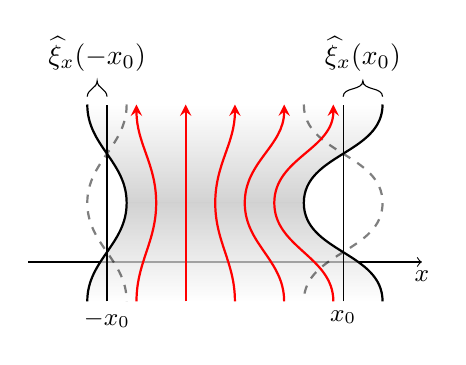
\begin{tikzpicture}
\draw [->] (1,0) -- (6,0);

\shade[bottom color=lightgray,top color=white, opacity=0.7] (1.75,2) to [out=-90,in=90] (2.25,0.75) to (4.5,0.75) to [out=90,in=-90] (5.5,2) to (1.75,2);

\shade[bottom color=white,top color=lightgray, opacity=0.7] (2.25,0.75) to (4.5,0.75) to [out=-90,in=90] (5.5,-0.5) to (1.75,-0.5) to [out=90,in=-90] (2.25,0.75);

\draw [thick] (1.75,2) to [out=-90,in=90] (2.25,0.75) to [out=-90,in=90] (1.75,-0.5);
\draw [thick, dashed, opacity=0.5] (4.5,2) to [out=-90,in=90] (5.5,0.75) to [out=-90,in=90] (4.5,-0.5);

\draw [thick, red, -stealth] (2.375,-0.5) to [out=90,in=-90] (2.625, 0.75) to [out=90,in=-90] (2.375,2);
\draw [thick, red, -stealth] (3,-0.5) to [out=90,in=-90] (3, 0.75) to [out=90,in=-90] (3,2);
\draw [thick, red, -stealth] (3.625,-0.5) to [out=90,in=-90] (3.375, 0.75) to [out=90,in=-90] (3.625,2);
\draw [thick, red, -stealth] (4.25,-0.5) to [out=90,in=-90] (3.75, 0.75) to [out=90,in=-90] (4.25,2);
\draw [thick, red, -stealth] (4.875,-0.5) to [out=90,in=-90] (4.125, 0.75) to [out=90,in=-90] (4.875,2);

\draw [thick, dashed, opacity=0.5] (2.25,2) to [out=-90,in=90] (1.75,0.75) to [out=-90,in=90] (2.25,-0.5);
\draw [thick] (5.5,2) to [out=-90,in=90] (4.5,0.75) to [out=-90,in=90] (5.5,-0.5);

% % % % % % % % % % % % % % % % % % % % % % % % % %

%\draw [->] (0,0) -- (0,2);

%\node at (1,1) {$\rho_1$};
%\node at (6,1) {$\rho_2$};
%\node [right] at (2.95,1.3) {$\rho_0$};

\draw [-] (1.75, 2.1) to [out=90, in=-90] (1.875, 2.3) to [out=-90, in=90] (2, 2.1);
\draw [-] (5, 2.1) to [out=90, in=-90] (5.25, 2.3) to [out=-90, in=90] (5.5, 2.1);

\node [above] at (1.875,2.3) {$\widehat{\xi}_x(-x_0)$};
\node [above] at (5.25, 2.3) {$\widehat{\xi}_x(x_0)$};

\small
\node [below] at (2,-0.5) {$-x_0$};
\node [below] at (5,-0.5) {$x_0$};

%\node [left] at (0,2) {$z$};
\node [below] at (6,0) {$x$};
\draw [-] (2,-0.5) -- (2,2);
\draw [-] (5,-0.5) -- (5,2);
\end{tikzpicture}
}}


\subfloat[]{\scalebox{0.9}{
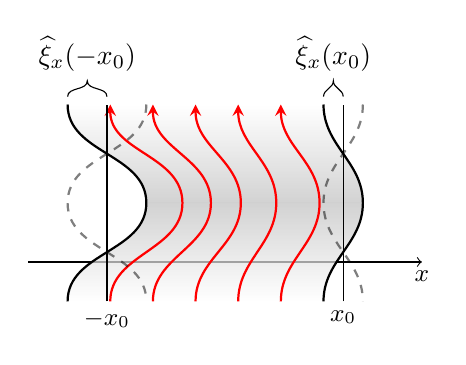
\begin{tikzpicture}
\draw [->] (1,0) -- (6,0);

\shade[bottom color=lightgray,top color=white, opacity=0.7] (1.5,2) to [out=-90,in=90] (2.5,0.75) to (5.25,0.75) to [out=90,in=-90] (4.75,2) to (1.5,2);

\shade[bottom color=white,top color=lightgray, opacity=0.7] (2.5,0.75) to (5.25,0.75) to [out=-90,in=90] (4.75,-0.5) to (1.5,-0.5) to [out=90,in=-90] (2.5,0.75);

\draw [thick] (1.5,2) to [out=-90,in=90] (2.5,0.75) to [out=-90,in=90] (1.5,-0.5);
\draw [thick] (4.75,2) to [out=-90,in=90] (5.25,0.75) to [out=-90,in=90] (4.75,-0.5);

%\draw [thick, red, -stealth] (2.0417,-0.5) to [out=90,in=-90] (2.9583, 0.75) to [out=90,in=-90] (2.0417,2);
%\draw [thick, red, -stealth] (2.5833,-0.5) to [out=90,in=-90] (3.4167, 0.75) to [out=90,in=-90] (2.5833,2);
%\draw [thick, red, -stealth] (3.125,-0.5) to [out=90,in=-90] (3.875, 0.75) to [out=90,in=-90] (3.125,2);
%\draw [thick, red, -stealth] (3.6667,-0.5) to [out=90,in=-90] (4.3333, 0.75) to [out=90,in=-90] (3.6667,2);
%\draw [thick, red, -stealth] (4.2083,-0.5) to [out=90,in=-90] (4.7917, 0.75) to [out=90,in=-90] (4.2083,2);

\draw [thick, red, -stealth] (2.0417,-0.5) to [out=90,in=-90] (2.9583, 0.75) to [out=90,in=-90] (2.0417,2);
\draw [thick, red, -stealth] (2.5833,-0.5) to [out=90,in=-90] (3.32, 0.75) to [out=90,in=-90] (2.5833,2);
\draw [thick, red, -stealth] (3.125,-0.5) to [out=90,in=-90] (3.7, 0.75) to [out=90,in=-90] (3.125,2);
\draw [thick, red, -stealth] (3.6667,-0.5) to [out=90,in=-90] (4.15, 0.75) to [out=90,in=-90] (3.6667,2);
\draw [thick, red, -stealth] (4.2083,-0.5) to [out=90,in=-90] (4.7, 0.75) to [out=90,in=-90] (4.2083,2);

\draw [thick, dashed, opacity=0.5] (2.5,2) to [out=-90,in=90] (1.5,0.75) to [out=-90,in=90] (2.5,-0.5);
\draw [thick, dashed, opacity=0.5] (5.25,2) to [out=-90,in=90] (4.75,0.75) to [out=-90,in=90] (5.25,-0.5);

% % % % % % % % % % % % % % % % % % % % % % % % % %

\draw [-] (1.5, 2.1) to [out=90, in=-90] (1.75, 2.3) to [out=-90, in=90] (2., 2.1);
\draw [-] (4.75, 2.1) to [out=90, in=-90] (4.875, 2.3) to [out=-90, in=90] (5., 2.1);

\node [above] at (1.75,2.3) {$\widehat{\xi}_x(-x_0)$};
\node [above] at (4.875, 2.3) {$\widehat{\xi}_x(x_0)$};

\small
\node [below] at (2,-0.5) {$-x_0$};
\node [below] at (5,-0.5) {$x_0$};

%\node [left] at (0,2) {$z$};
\node [below] at (6,0) {$x$};
\draw [-] (2,-0.5) -- (2,2);
\draw [-] (5,-0.5) -- (5,2);
\end{tikzpicture}
}}}
\caption{Illustration of the difference in amplitude of oscillation on each boundary of the slab for~(a)~quasi-sausage and~(b)~quasi-kink modes. The ratio of the amplitudes can be used as a diagnostic tool.}
\label{fig: RA}
\end{figure}

We now define the \emph{amplitude ratio}, $R_\textrm{A} := \widehat{\xi}_x(x_0) / \widehat{\xi}_x(-x_0)$, as the ratio of the amplitude of oscillation of the left interface ($x=x_0$) to that of the right interface ($x=-x_0$) (Figure~\ref{fig: RA}). Given that ${\widehat{\xi}_x(x) = i\widehat{v}_x(x) / \omega}$, we also have $R_\textrm{A} = \widehat{v}_x(x_0) / \widehat{v}_x(-x_0)$. Firstly, using equations~\eqref{v-x_01 C} and \eqref{vx_02 C}, the amplitude ratio for quasi-sausage modes is
\begin{align}
R_A &=-\frac{\Lambda_0+\Lambda_1\frac{1}{\tau_0}}{\Lambda_0+\Lambda_2\frac{1}{\tau_0}} \notag \\
	&=-\frac{\rho_1m_2}{\rho_2m_1}\left[\frac{(k^2v_\textrm{A}^2-\omega^2)m_1\frac{\rho_0}{\rho_1}-\omega^2m_0\frac{1}{\tanh{m_0x_0}}}{(k^2v_\textrm{A}^2-\omega^2)m_2\frac{\rho_0}{\rho_2}-\omega^2m_0\frac{1}{\tanh{m_0x_0}}}\right]. \label{cross-slab ratio saus}
\end{align}
Using equations~\eqref{v-x_01 B} and~\eqref{vx_02 B}, the corresponding expression for quasi-kink modes can be obtained, namely
\begin{align}
R_\textrm{A}&=\frac{\Lambda_0+\Lambda_1\tau_0}{\Lambda_0+\Lambda_2\tau_0} \notag \\
	&=\frac{\rho_1m_2}{\rho_2m_1}\left[\frac{(k^2v_\textrm{A}^2-\omega^2)m_1\frac{\rho_0}{\rho_1}-\omega^2m_0\tanh{m_0x_0}}{(k^2v_\textrm{A}^2-\omega^2)m_2\frac{\rho_0}{\rho_2}-\omega^2m_0\tanh{m_0x_0}}\right]. \label{cross-slab ratio kink}
\end{align}
As expected, equations \eqref{cross-slab ratio saus} and \eqref{cross-slab ratio kink} reduce to $R_\textrm{A} = -1$ and $R_\textrm{A} = 1$ for sausage and kink modes, respectively, when the slab is symmetric.

The following subsections give the analytical solution for the Alfv\'{e}n speed, $v_\textrm{A}$, of equations~\eqref{cross-slab ratio saus} and~\eqref{cross-slab ratio kink} under the thin slab, wide slab, incompressible plasma, and low-beta approximations. To obtain an approximation for the Alfv\'{e}n speed analytically, an approximation such as these must be applied. Note that we restrict the analysis to surface modes only, thereby omitting body modes, because the eigenfrequencies and eigenfunctions of body modes are not significantly effected by asymmetry in the external plasma \citep{all_etal17}.


\subsection{Thin slab approximation} \label{sec: AR thin slab}
In the thin slab approximation, $kx_0 \ll 1$, it has been shown that $m_0x_0 \ll 1$ for surface modes \citep{rob81b}. Therefore, $\tanh{m_0x_0} \approx m_0x_0$ and the amplitude ratio for a quasi-sausage surface mode in a thin slab reduces to
\begin{equation}
R_\textrm{A} = -\frac{\rho_1m_2}{\rho_2m_1}\left[\frac{(k^2v_\textrm{A}^2-\omega^2)m_1x_0\frac{\rho_0}{\rho_1}-\omega^2}{(k^2v_\textrm{A}^2-\omega^2)m_2x_0\frac{\rho_0}{\rho_2}-\omega^2}\right], 
\end{equation}
which has analytical solutions
\begin{equation}
v_\textrm{A}^2 = \frac{\omega^2}{k^2} \left[1 + \frac{1}{x_0}\left(\frac{R_\textrm{A}\frac{\rho_2}{\rho_0m_2} + \frac{\rho_1}{\rho_0m_1}}{R_\textrm{A} + 1}\right)\right].
\end{equation}
The amplitude ratio for a thin slab quasi-kink surface mode reduces to
\begin{equation}
R_\textrm{A} = \frac{\rho_1m_2}{\rho_2m_1}\left[\frac{(k^2v_\textrm{A}^2-\omega^2)m_1\frac{\rho_0}{\rho_1}-\omega^2m_0^2x_0}{(k^2v_\textrm{A}^2-\omega^2)m_2\frac{\rho_0}{\rho_2}-\omega^2m_0^2x_0}\right], 
\end{equation}
which has analytical solutions
\begin{equation}
v_\textrm{A}^2 = \frac{\omega^2}{k^2} \left[\frac{c_0^2}{c_0^2 - \frac{\omega^2}{k^2}} + k^2x_0\left(\frac{R_\textrm{A}\frac{\rho_2}{\rho_0m_2} - \frac{\rho_1}{\rho_0m_1}}{R_\textrm{A} - 1}\right)\right]. \label{AR soln kink thin}
\end{equation}

In a thin asymmetric slab, the fast quasi-kink surface mode degenerates due to a cut-off by the external sound speeds becoming distinct \citep{all_etal17} and the slow quasi-kink surface mode has a phase speed that approaches zero in the thin slab limit. Therefore, to a good approximation, the phase speed is much less than the internal sound speed ($\omega/k \ll c_0$) therefore Solution~\eqref{AR soln kink thin} simplifies to
\begin{equation}
v_\textrm{A}^2 = \frac{\omega^2}{k^2} \left[1 + k^2x_0\left(\frac{R_\textrm{A}\frac{\rho_2}{\rho_0m_2} - \frac{\rho_1}{\rho_0m_1}}{R_\textrm{A} - 1}\right)\right]. \label{AR soln kink thin simplified}
\end{equation}

\subsection{Wide slab approximation} \label{sec: AR wide slab}
The wide slab approximation applies when the slab width is much larger than the wavelength, that is $kx_0 \gg 1$. To understand the properties of the eigenfunctions of the asymmetric slab system in the wide slab approximation, we must return to the dispersion relation, Equation~\eqref{disp rel}. For surface modes in the slab, the wide slab approximation implies that $m_0x_0 \gg 1$, therefore ${\sinh{m_0x_0} \approx \cosh{m_0x_0} \approx 1}$ \citep{rob81b}. Under this approximation, the dispersion relation, Equation~\eqref{disp rel}, becomes
\begin{equation}
(\Lambda_0 + \Lambda_1)(\Lambda_0 + \Lambda_2) = 0,
\end{equation}
which gives us two families of solutions, one satisfying $\Lambda_0 + \Lambda_1 = 0$ and the other satisfying $\Lambda_0 + \Lambda_2 = 0$. These are equivalent to
\begin{equation}
(k^2v_\textrm{A}^2 - \omega^2)m_j\frac{\rho_0}{\rho_j} - \omega^2m_0 = 0,
\end{equation}
for $j = 1, 2$, respectively. This equation is the same as the dispersion relation governing surface waves along a single interface between a magnetised and a non-magnetised plasma \citep{rob81a}. Hence, the surface mode solutions of a wide asymmetric slab are just the surface modes that propagate along each interface independently. This makes intuitive sense considering that as the slab is widened the interfaces will have diminishing influence on each other, until each interface oscillates independently with its own characteristic frequency.

This is analogous to the mechanical example introduced by \citealp{all_etal17}. Consider two masses connected by a spring, with spring constant $k_0$, and each mass is also connected to a fixed wall on each side by springs with spring constants $k_1$ and $k_2$, respectively (Figure~\ref{fig: wide slab mechanical analogy}). When the middle spring has spring constant $k_0 \neq 0$, there are two modes, an in-phase mode (analogous to kink modes in a slab) and an in-antiphase mode (analogous to sausage modes in a slab) \citep{all_etal17}. When the two masses are decoupled by removing the middle spring, equivalently setting $k_0 = 0$, each mass oscillates independently at the natural frequency of that side of the spring-mass system. This decoupling provides a good analogy to the wide slab limit for the magnetic slab. Each interface can oscillate at its own natural frequency, independent of the other interface. Given that we are considering magneto-acoustic waves, there are two restoring forces, the magnetic tension force and the pressure gradient force, which means that each independent interface has two natural frequencies (depending on the parameters of the system, there can be 0, 1, or 2 frequencies), corresponding to the fast and slow magneto-acoustic modes.

With this understanding of the modes in the wide slab limit, the amplitude ratio, $R_\textrm{A}$, is either $0$ or \textit{undefined}, depending on which interface the wave is propagating and is therefore not useful for magneto-seismology.

\begin{figure}
\makebox[\textwidth][c]{
\subfloat[Coupled equilibrium]{\scalebox{0.9}{
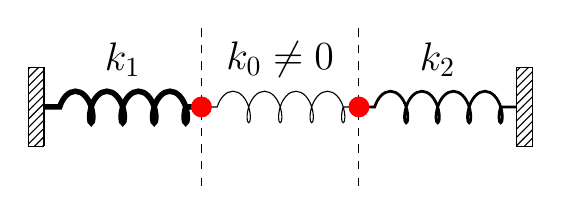
\begin{tikzpicture}
\filldraw[pattern=north east lines] (0,-0.5) -| (-0.2,0.5) -| (0,-0.5);
\filldraw[pattern=north east lines] (6,-0.5) -| (6.2,0.5) -| (6,-0.5);
\draw[Spring, line width=2] (0,0) -- (2,0);
\draw[Spring, thin] (2,0) -- (4,0);
\draw[Spring, line width=1] (4,0) -- (6,0);

\draw [dashed] (2,1) -- (2,-1);
\draw [dashed] (4,1) -- (4,-1);

\draw (2,0) node [fill=red,circle,scale=0.8] {};
\draw (4,0) node [fill=red,circle,scale=0.8] {};

\Large
\draw (1,0.6) node [] {$k_1$};
\draw (3,0.6) node [] {$k_0 \neq 0$};
\draw (5,0.6) node [] {$k_2$};
\end{tikzpicture}
}}

\subfloat[Uncoupled equilibrium]{\scalebox{0.9}{
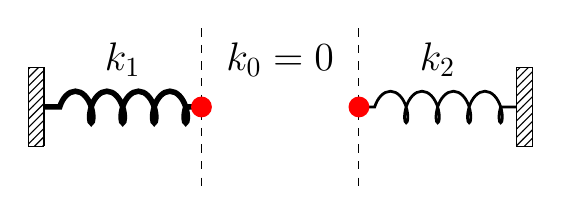
\begin{tikzpicture}
\filldraw[pattern=north east lines] (0,-0.5) -| (-0.2,0.5) -| (0,-0.5);
\filldraw[pattern=north east lines] (6,-0.5) -| (6.2,0.5) -| (6,-0.5);
\draw[Spring, line width=2] (0,0) -- (2,0);
%\draw[Spring, thin] (2,0) -- (4,0);
\draw[Spring, line width=1] (4,0) -- (6,0);

\draw [dashed] (2,1) -- (2,-1);
\draw [dashed] (4,1) -- (4,-1);

\draw (2,0) node [fill=red,circle,scale=0.8] {};
\draw (4,0) node [fill=red,circle,scale=0.8] {};

\Large
\draw (1,0.6) node [] {$k_1$};
\draw (3,0.6) node [] {$k_0 = 0$};
\draw (5,0.6) node [] {$k_2$};
\end{tikzpicture}
}}}

\makebox[\textwidth][c]{
\subfloat[Uncoupled left oscillation]{\scalebox{0.9}{
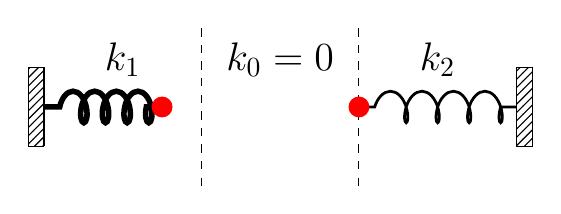
\begin{tikzpicture}
\filldraw[pattern=north east lines] (0,-0.5) -| (-0.2,0.5) -| (0,-0.5);
\filldraw[pattern=north east lines] (6,-0.5) -| (6.2,0.5) -| (6,-0.5);
\draw[Spring, line width=2] (0,0) -- (1.5,0);
%\draw[Spring, thin] (2,0) -- (4,0);
\draw[Spring, line width=1] (4,0) -- (6,0);

\draw [dashed] (2,1) -- (2,-1);
\draw [dashed] (4,1) -- (4,-1);

\draw (1.5,0) node [fill=red,circle,scale=0.8] {};
\draw (4,0) node [fill=red,circle,scale=0.8] {};

\Large
\draw (1,0.6) node [] {$k_1$};
\draw (3,0.6) node [] {$k_0 = 0$};
\draw (5,0.6) node [] {$k_2$};
\end{tikzpicture}
}}

\subfloat[Uncoupled right oscillation]{\scalebox{0.9}{
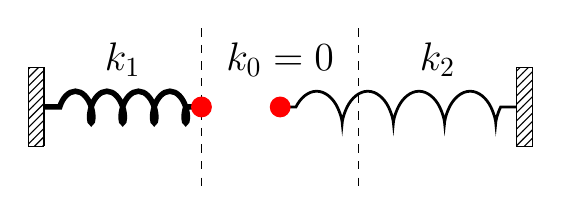
\begin{tikzpicture}
\filldraw[pattern=north east lines] (0,-0.5) -| (-0.2,0.5) -| (0,-0.5);
\filldraw[pattern=north east lines] (6,-0.5) -| (6.2,0.5) -| (6,-0.5);
\draw[Spring, line width=2] (0,0) -- (2,0);
%\draw[Spring, thin] (2,0) -- (4,0);
\draw[Spring, line width=1] (3,0) -- (6,0);

\draw [dashed] (2,1) -- (2,-1);
\draw [dashed] (4,1) -- (4,-1);

\draw (2,0) node [fill=red,circle,scale=0.8] {};
\draw (3,0) node [fill=red,circle,scale=0.8] {};

\Large
\draw (1,0.6) node [] {$k_1$};
\draw (3,0.6) node [] {$k_0 = 0$};
\draw (5,0.6) node [] {$k_2$};
\end{tikzpicture}
}}}
\caption{Mechanical example showing weak and zero coupling between the masses. This provides an analogy to the wide slab approximation of an asymmetric magnetic slab, in which case the interfaces on each side of the slab oscillate independently.}
\label{fig: wide slab mechanical analogy}
\end{figure}

\subsection{Incompressible Approximation} \label{sec: AR incomp}

If the plasma in each region is incompressible, the sound speeds become unbounded, so that $m_j \approx k$ for $j = 0,1,2$. Under this approximation, the amplitude ratio for quasi-sausage modes (top) and quasi-kink modes (bottom) reduces to
\begin{align}
R_\textrm{A} &= \left(\substack{- \\ +}\right) \frac{\rho_1}{\rho_2} \left[ \frac{(k^2v_\textrm{A}^2-\omega^2)k\frac{\rho_0}{\rho_1}-\omega^2k \left(\hspace{-0.07in}\begin{matrix} &\coth \\ &\tanh \end{matrix}\right)(kx_0)}{(k^2v_\textrm{A}^2-\omega^2)k\frac{\rho_0}{\rho_2}-\omega^2k \left(\hspace{-0.07in}\begin{matrix} &\coth \\ &\tanh \end{matrix}\right)(kx_0)} \right].
\end{align}
These equations have solutions for $v_\textrm{A}$ given by
\begin{equation}
v_\textrm{A}^2 = \frac{\omega^2}{k^2} \left[ 1 + \left( \frac{R_\textrm{A} \frac{\rho_2}{\rho_0} \left(\substack{+ \\ -}\right) \frac{\rho_1}{\rho_0}}{R_\textrm{A} \left(\substack{+ \\ -}\right) 1} \right) \left(\hspace{-0.07in}\begin{matrix} &\coth \\ &\tanh \end{matrix}\right) (kx_0)\right].
\end{equation}

\subsection{Low-Beta Approximation} \label{sec: AR low-beta}

For a low-beta plasma ($\beta = 2\mu_0p_0/B_0^2 \ll 1$), where the magnetic pressure dominates the plasma pressure, the Alfv\'{e}n speed, $v_\textrm{A}$, dominates the internal sound speed, $c_0$, so that $m_0^2 \approx k^2-\omega^2/v_\textrm{A}^2$. For waves with phase speed much less than the Alfv\'{e}n speed, a further approximation of $m_0^2 \approx k^2$ can be made, in which case the amplitude ratio for quasi-sausage modes (top) and quasi-kink modes (bottom) reduces to
\begin{align}
R_\textrm{A} &= \left(\substack{- \\ +}\right) \frac{\rho_1m_2}{\rho_2m_1} \left[ \frac{(k^2v_\textrm{A}^2-\omega^2)m_1\frac{\rho_0}{\rho_1}-\omega^2k \left(\hspace{-0.07in}\begin{matrix} &\coth \\ &\tanh \end{matrix}\right)(kx_0)}{(k^2v_\textrm{A}^2-\omega^2)m_2\frac{\rho_0}{\rho_2}-\omega^2k \left(\hspace{-0.07in}\begin{matrix} &\coth \\ &\tanh \end{matrix}\right)(kx_0)} \right].
\end{align}
These equations can be solved for $v_\textrm{A}$ to give
\begin{equation}
v_\textrm{A}^2 = \frac{\omega^2}{k^2} \left[1 + k \left( \frac{ \frac{\rho_1}{\rho_0m_1} \left(\substack{+ \\ -}\right) R_\textrm{A}\frac{\rho_2}{\rho_0m_2}}{1 \left(\substack{+ \\ -}\right) R_\textrm{A}} \right) \left(\hspace{-0.07in}\begin{matrix} &\coth \\ &\tanh \end{matrix}\right) (kx_0)\right].
\end{equation}

We will return to a discussion of the inversion of the amplitude ratio in Section~\ref{sec: discussion}.


%BELOW APPROXIMATION DOES NOT RETAIN MAGNETIC FIELD, SO IS WORTHLESS, PROBABLY.

%\subsection{Approximately Equal External Parameters} \label{sec: approx equal parameters}
%If the parameters of the non-magnetised external regions agree to first order approximation, the dispersion relation for magneto-acoustic waves along an asymmetric slab reduces to
%\begin{align}
%&\Lambda_0(\Lambda_1+\Lambda_2)+2\Lambda_1\Lambda_2\tau_0=0, \label{DR saus} \\
%&\Lambda_0(\Lambda_1+\Lambda_2)+2\Lambda_1\Lambda_2\frac{1}{\tau_0}=0, \label{DR kink}
%\end{align}
%for quasi-sausage and quasi-kink modes, respectively. Manipulation of equation~\eqref{DR saus} yields
%\begin{align}
%\Lambda_0\Lambda_1+\Lambda_1\Lambda_2\tau_0&=-(\Lambda_0\Lambda_2+\Lambda_1\Lambda_2\tau_0), \\
%\implies
%\Lambda_1(\Lambda_0+\Lambda_2\tau_0)&=-\Lambda_2(\Lambda_0+\Lambda_1\tau_0), \\
%\implies \frac{\Lambda_0+\Lambda_1\tau_0}{\Lambda_0+\Lambda_2\tau_0}&=-\frac{\Lambda_1}{\Lambda_2}=-\frac{\rho_1m_2}{\rho_2m_1}.
%\end{align}
%Similar manipulation of equation~\eqref{DR kink} yields
%\begin{equation}
%\frac{\Lambda_0\tau_0+\Lambda_1}{\Lambda_0\tau_0+\Lambda_2}=-\frac{\Lambda_1}{\Lambda_2}=-\frac{\rho_1m_2}{\rho_2m_1}.
%\end{equation}
%If the conditions on either side of the slab are equal to first order approximation, the cross-slab amplitude ratio reduces to
%\begin{equation}
%R_\textrm{A}=-\frac{\rho_1m_2}{\rho_2m_1}, \label{cross-slab ratio approx saus}
%\end{equation}
%for quasi-sausage modes, and
%\begin{equation}
%R_\textrm{A}=\frac{\rho_1m_2}{\rho_2m_1}, \label{cross-slab ratio approx kink}
%\end{equation}
%for quasi-kink modes.


\section{Shift of minimum perturbation}
A second spatial seismology technique uses the shift in the position of minimum wave power from the centre of the slab due to the asymmetry in the external plasma regions as a diagnostic parameter for the slab Alfv\'{e}n speed.

The position of minimum wave power for a symmetric sausage or kink mode is at the central line of the slab, at $x=0$. We define $\Delta_\textrm{min}$ to be the displacement (from the central line) of the position of minimum wave power inside an asymmetric magnetic slab. For quasi-sausage modes, $\Delta_\textrm{min}$ is the solution to $\widehat{v}_x(x) = 0$ under the constraint $|x| < x_0$, and for quasi-kink modes, $\Delta_\textrm{min}$ is the solution to $\textrm{d}\widehat{v}_x (x) / \textrm{d}x = 0$ under the same constraint $|x| < x_0$. The constraint restricts the solutions to being within the slab. 

\begin{figure}
\makebox[\textwidth][c]{
\subfloat[]{\scalebox{0.9}{
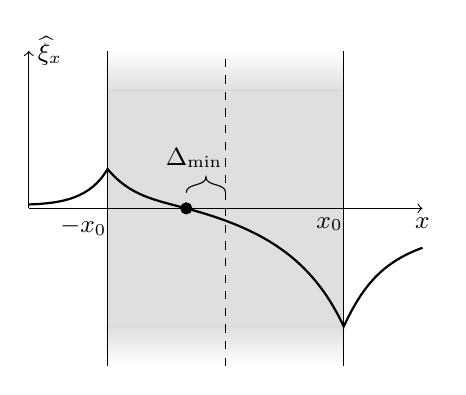
\begin{tikzpicture}
\path [fill=lightgray, opacity=0.5] (2,-1.5) -- (2,1.5) -- (5,1.5) -- (5,-1.5) -- (2,-1.5);

\shade[bottom color=white,top color=lightgray, opacity=0.5] (2,-2) to (5,-2) to (5,-1.5) to (2,-1.5) to (2,-2);

\shade[top color=white,bottom color=lightgray, opacity=0.5] (2,2) to (5,2) to (5,1.5) to (2,1.5) to (2,2);

\draw [-] (2,-2) -- (2,2);
\draw [-] (5,-2) -- (5,2);

%\draw [ultra thick, red, -stealth,opacity=0.7] (2.5,-1.5) -- (2.5,2);
%\draw [ultra thick, red, path fading=south, opacity=0.5] (2.5,-2) -- (2.5,-1.5);
%\draw [ultra thick, red, -stealth,opacity=0.7] (3,-1.5) -- (3,2);
%\draw [ultra thick, red, path fading=south,opacity=0.5] (3,-2) -- (3,-1.5);
%\draw [ultra thick, red, -stealth,opacity=0.7] (3.5,-1.5) -- (3.5,2);
%\draw [ultra thick, red, path fading=south,opacity=0.5] (3.5,-2) -- (3.5,-1.5);
%\draw [ultra thick, red, -stealth,opacity=0.7] (4,-1.5) -- (4,2);
%\draw [ultra thick, red, path fading=south,opacity=0.5] (4,-2) -- (4,-1.5);
%\draw [ultra thick, red, -stealth,opacity=0.7] (4.5,-1.5) -- (4.5,2);
%\draw [ultra thick, red, path fading=south,opacity=0.5] (4.5,-2) -- (4.5,-1.5);

%\draw [thick] (0,0.025) to [out=0, in=-178] (1.2, 0.05) to [out=2, in=-120] (2,0.5) to [out=-50, in=165] (3,0) to [out=-15, in=115] (5,-1.5) to [out=65, in=-170] (7,-0.2);

\draw [thick] (1, 0.05) to [out=2, in=-120] (2,0.5) to [out=-50, in=165] (3,0) to [out=-15, in=115] (5,-1.5) to [out=65, in=-160] (6,-0.5);

\draw [->] (1,0) -- (1,2);
\draw [->] (1,0) -- (6,0);

%\node at (1,1) {$\rho_1$};
%\node at (6,1) {$\rho_2$};
%\node [right] at (2.88,1.3) {$\rho_0$};

\small
\node [below left] at (2.1,0) {$-x_0$};
\node [below left] at (5.1,0) {$x_0$};

\node [right] at (1,2) {$\widehat{\xi}_x$};
\node [below] at (6,0) {$x$};

\draw [dashed] (3.5,-2) -- (3.5,2);
\draw [fill] (3,0) circle [radius=0.07];
\draw [-] (3, 0.2) to [out=90, in=-90] (3.25, 0.4) to [out=-90, in=90] (3.5, 0.2);
\node [above] at (3.1, 0.4) {$\Delta_\mathrm{min}$};
\end{tikzpicture}
}}


\subfloat[]{\scalebox{0.9}{
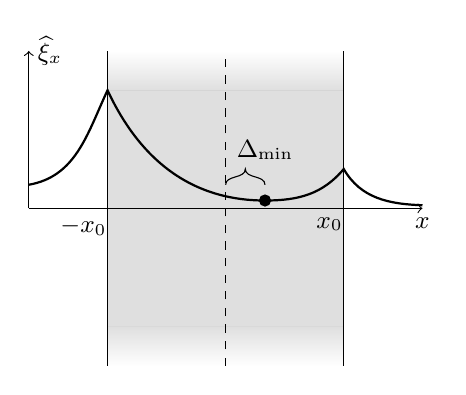
\begin{tikzpicture}
\path [fill=lightgray, opacity=0.5] (2,-1.5) -- (2,1.5) -- (5,1.5) -- (5,-1.5) -- (2,-1.5);

\shade[bottom color=white,top color=lightgray, opacity=0.5] (2,-2) to (5,-2) to (5,-1.5) to (2,-1.5) to (2,-2);

\shade[top color=white,bottom color=lightgray, opacity=0.5] (2,2) to (5,2) to (5,1.5) to (2,1.5) to (2,2);

\draw [-] (2,-2) -- (2,2);
\draw [-] (5,-2) -- (5,2);

%\draw [ultra thick, red, -stealth,opacity=0.7] (2.5,-1.5) -- (2.5,2);
%\draw [ultra thick, red, path fading=south, opacity=0.5] (2.5,-2) -- (2.5,-1.5);
%\draw [ultra thick, red, -stealth,opacity=0.7] (3,-1.5) -- (3,2);
%\draw [ultra thick, red, path fading=south,opacity=0.5] (3,-2) -- (3,-1.5);
%\draw [ultra thick, red, -stealth,opacity=0.7] (3.5,-1.5) -- (3.5,2);
%\draw [ultra thick, red, path fading=south,opacity=0.5] (3.5,-2) -- (3.5,-1.5);
%\draw [ultra thick, red, -stealth,opacity=0.7] (4,-1.5) -- (4,2);
%\draw [ultra thick, red, path fading=south,opacity=0.5] (4,-2) -- (4,-1.5);
%\draw [ultra thick, red, -stealth,opacity=0.7] (4.5,-1.5) -- (4.5,2);
%\draw [ultra thick, red, path fading=south,opacity=0.5] (4.5,-2) -- (4.5,-1.5);

%\draw [thick] (0,0.2) to [out=10, in=245] (2, 1.5) to [out=295, in=180] (4,0.1) to [out=0, in=230] (5,0.5) to [out=300, in=178] (6.2,0.04) to [out=358, in=180] (7,0.02);

\draw [thick] (1,0.3) to [out=10, in=245] (2, 1.5) to [out=295, in=180] (4,0.1) to [out=0, in=230] (5,0.5) to [out=300, in=178] (6,0.04);

\draw [->] (1,0) -- (1,2);
\draw [->] (1,0) -- (6,0);
%
%\node at (1,1) {$\rho_1$};
%\node at (6,1) {$\rho_2$};
%\node [right] at (2.88,1.3) {$\rho_0$};

\small
\node [below left] at (2.1,0) {$-x_0$};
\node [below left] at (5.1,0) {$x_0$};

\node [right] at (1,2) {$\widehat{\xi}_x$};
\node [below] at (6,0) {$x$};

\draw [dashed] (3.5,-2) -- (3.5,2);
\draw [fill] (4,0.1) circle [radius=0.07];
\draw [-] (3.5, 0.3) to [out=90, in=-90] (3.75, 0.5) to [out=-90, in=90] (4, 0.3);
\node [above] at (4, 0.5) {$\Delta_\mathrm{min}$};
\end{tikzpicture}
}}}

\caption{Illustration of the minimum perturbation shift within the slab for (a) quasi-sausage and (b) quasi-kink modes. The minimum perturbation shift can be used as a diagnostic tool.}
\end{figure}

Firstly, for quasi-sausage modes, using the solution for the transversal velocity amplitude given by Equation~\eqref{vsoln} and the expressions for the variables within given by equation~\eqref{constB C}, the shift of minimum perturbation can be calculated as follows. The solution for the transversal velocity amplitude within the slab is
\begin{equation}
\widehat{v}_x(x) = B\cosh{m_0x}+C\sinh{m_0x} = 0,
\end{equation}
where $B$ is given by equation~\eqref{constB C} and $C$ is arbitrary. This equation is solved for $x$ to give
\begin{equation}
x = \frac{1}{m_0} \tanh^{-1}\left(-\frac{B}{C}\right). \label{disp of min power saus}
\end{equation}
therefore the shift of minimum perturbation is
\begin{equation}
\Delta_\textrm{min} = \frac{1}{m_0}\tanh^{-1}\left(-\frac{(k^2{v_\textrm{A}}^2-\omega^2)m_1\frac{\rho_0}{\rho_1} - \omega^2{m_0}\tanh{m_0x_0}}{(k^2{v_\textrm{A}}^2-\omega^2)m_1\frac{\rho_0}{\rho_1}\tanh{m_0x_0} - \omega^2{m_0}}\right). \label{shift min saus}
\end{equation}
Similarly, for quasi-kink modes, using Equations~\eqref{vsoln} and \eqref{constB B} we calculate the shift of minimum perturbation to be
\begin{equation}
\Delta_\textrm{min} = \frac{1}{m_0}\coth^{-1}\left(-\frac{(k^2{v_\textrm{A}}^2-\omega^2)m_1\frac{\rho_0}{\rho_1} - \omega^2{m_0}\tanh{m_0x_0}}{(k^2{v_\textrm{A}}^2-\omega^2)m_1\frac{\rho_0}{\rho_1}\tanh{m_0x_0} - \omega^2{m_0}}\right). \label{shift min kink}
\end{equation}

It appears that expressions~\eqref{shift min saus} and~\eqref{shift min kink} for the minimum perturbation shifts depend on the parameters in the slab (subscript~0), the left external plasma (subscript~1), but not on the parameters of the right external plasma (subscript~2). However, the dependence on the right external plasma is implicit in the determination of the eigenfrequency $\omega$ when solving the dispersion relation.

The concept of minimum perturbation shift is exclusive to surface modes. The eigenfunctions of surface modes in a magnetic slab depend much more on the plasma parameters, such as the density, than body modes \citep{all_etal17}. This makes intuitive sense given that the energy in a surface mode is localised to the boundaries of the slab whereas the energy in a body mode is largely isolated within the slab. There is a quantifiable shift in the spatial nodes and anti-nodes in body mode perturbations within a slab due to changing external plasma parameters, however it is so small that is would not be an effective observational tool.

Akin to the amplitude ratio method for solar magneto-seismology prescribed in Section~\ref{sec: AR}, we can solve equation~\eqref{shift min saus} or~\eqref{shift min kink} for the Alfv\'{e}n speed, $v_\textrm{A}$, to achieve an approximation for the magnetic field strength of inhomogeneous solar magnetic structures. This can be done either numerically, using an iterative root finding method, or analytically, under an appropriate approximation, as discussed below.


\subsection{Thin slab approximation}
As noted in Section~\ref{sec: AR thin slab}, for surface modes, the thin slab limit, that is $kx_0 \ll 1$, implies $m_0x_0 \ll 1$. By definition $\Delta_\textrm{min} < x_0$, therefore $m_0\Delta_{min} \ll 1$, so that $\tanh{m_0\Delta_\textrm{min}} \approx m_0\Delta_\textrm{min}$. Firstly, for quasi-sausage modes, Equation~\eqref{shift min saus} can be solved for $v_\textrm{A}$ to give
\begin{equation}
v_\textrm{A}^2 = \frac{\omega^2}{k^2} \left[\frac{\rho_1}{\rho_0m_1}(x_0 + \Delta_\textrm{min}) + \frac{1}{1 + (\omega / kc_0)^2} + k^2x_0\Delta_\textrm{min}\right].
\end{equation}
For quasi-kink modes in a thin slab, Equation~\eqref{shift min kink} can be solved for $v_\textrm{A}$ to give
\begin{equation}
v_\textrm{A}^2 = \frac{\omega^2}{k^2}\left[\frac{-b \pm \sqrt{b^2 - 4ac}}{2a}\right],
\end{equation}
where
\begin{align}
a &= m_1\frac{\rho_0}{\rho_1}(k^2c_0^2 - \omega^2)(x_0 + \Delta_\textrm{min}), \\
b &= -m_1\frac{\rho_0}{\rho_1}(2k^2c_0^2 - \omega^2)(x_0 + \Delta_\textrm{min}) - (k^2c_0^2 - \omega^2), \\
c &= c_0^2m_1\frac{\rho_0}{\rho_1}(x_0 + \Delta_\textrm{min}) + c_0^2 + \omega^2x_0\Delta_\textrm{min}.
\end{align}


\subsection{Wide slab approximation}
The concept of minimum perturbation shift is ill-defined under the wide slab approximation. In the wide slab approximation, each interface oscillates independently at its own eigenfrequency. Therefore the nomenclature of quasi-sausage and quasi-kink mode breaks down. In the wide slab limit, the eigenfunctions have no local minimum in the slab, instead the perturbations are evanescent away from the interface that the oscillation is localised, therefore there is no locally minimum wave power within the slab.


\subsection{Incompressible approximation}
When the plasma is incompressible, the sound speeds are unbounded, so that $m_j = k$, for $j = 0, 1, 2$. The minimum perturbation shift for a quasi-sausage mode (top) and quasi-kink (bottom) in an incompressible slab is
\begin{equation}
\Delta_\textrm{min} = \frac{1}{k}\left(\hspace{-0.07in}\begin{matrix} &\tanh^{-1} \\ &\coth^{-1} \end{matrix}\right)\left(-\frac{(k^2{v_\textrm{A}}^2-\omega^2)\frac{\rho_0}{\rho_1} - \omega^2\tanh{kx_0}}{(k^2{v_\textrm{A}}^2-\omega^2)\frac{\rho_0}{\rho_1}\tanh{kx_0} - \omega^2}\right),
\end{equation}
which can be solved for $v_\textrm{A}$ to give
\begin{equation}
v_\textrm{A}^2 = \frac{\omega^2}{k^2}\left[1 + \frac{\rho_1}{\rho_0}\left(\hspace{-0.07in}\begin{matrix} &\tanh \\ &\coth \end{matrix}\right)(k(x_0 + \Delta_\textrm{min}))\right].
\end{equation}


\subsection{Low-beta approximation}
In a low-beta plasma, the minimum perturbation shift for a quasi-sausage mode (top) and quasi-kink (bottom) is given by
\begin{equation}
\Delta_\textrm{min} = \frac{1}{k}\left(\hspace{-0.07in}\begin{matrix} &\tanh^{-1} \\ &\coth^{-1} \end{matrix}\right)\left(-\frac{(k^2{v_\textrm{A}}^2-\omega^2)m_1\frac{\rho_0}{\rho_1} - \omega^2k\tanh{kx_0}}{(k^2{v_\textrm{A}}^2-\omega^2)m_1\frac{\rho_0}{\rho_1}\tanh{kx_0} - \omega^2k}\right),
\end{equation}
which can be solved for $v_\textrm{A}$ to give
\begin{equation}
v_\textrm{A}^2 = \frac{\omega^2}{k^2}\left[1 + \frac{k\rho_1}{m_1\rho_0}\left(\hspace{-0.07in}\begin{matrix} &\tanh \\ &\coth \end{matrix}\right)(k(x_0 + \Delta_\textrm{min}))\right].
\end{equation}

%\newgeometry{margin=1cm} % modify this if you need even more space
\begin{landscape}

\begin{table}
\caption{Magneto-seismological application using the amplitude ratio, $R_\textrm{A}$, to approximate the Alfv\'{e}n speed, $v_\textrm{A}$.}
\begin{tabular}{llccc}
  \toprule
Type & Mode & \multicolumn{3}{c}{Approximation of $k^2v_\textrm{A}^2 / \omega^2$ using amplitude ratio, $R_\textrm{A}$} \\
\cmidrule(lr){3-5}
	 &	    & \multicolumn{1}{c}{Thin slab} & \multicolumn{1}{c}{Incompressible} & \multicolumn{1}{c}{Low-beta} \\
  \midrule
\multirow{2}{*}{Surface} & Quasi-sausage & $ 1 + \frac{1}{x_0}\left(\frac{R_\textrm{A}\frac{\rho_2}{\rho_0m_2} + \frac{\rho_1}{\rho_0m_1}}{R_\textrm{A} + 1}\right) $ & $ 1 + \left( \frac{R_\textrm{A} \frac{\rho_2}{\rho_0} + \frac{\rho_1}{\rho_0}}{R_\textrm{A} + 1} \right) \coth{kx_0} $ & $ 1 + k \left( \frac{ R_\textrm{A}\frac{\rho_2}{\rho_0m_2} + \frac{\rho_1}{\rho_0m_1}}{R_\textrm{A} + 1} \right) \coth{kx_0} $ \\
						   & Quasi-kink	   & $ 1 + k^2x_0\left(\frac{R_\textrm{A}\frac{\rho_2}{\rho_0m_2} - \frac{\rho_1}{\rho_0m_1}}{R_\textrm{A} - 1}\right) $ & $ 1 + \left( \frac{R_\textrm{A} \frac{\rho_2}{\rho_0} - \frac{\rho_1}{\rho_0}}{R_\textrm{A} - 1} \right) \tanh{kx_0} $ & $ 1 + k \left( \frac{ R_\textrm{A}\frac{\rho_2}{\rho_0m_2} - \frac{\rho_1}{\rho_0m_1}}{R_\textrm{A} - 1} \right) \tanh{kx_0} $ \\
  \bottomrule
\end{tabular} \label{table: amp ratio}
\end{table}


\begin{table}
\caption{Magneto-seismological application using the minimum perturbation shift, $\Delta_\textrm{min}$, to approximate the Alfv\'{e}n speed, $v_\textrm{A}$.}
\begin{tabular}{llccc}
  \toprule
Type & Mode & \multicolumn{3}{c}{Approximation of $k^2v_\textrm{A}^2 / \omega^2$ using minimum perturbation shift, $\Delta_\textrm{min}$} \\
\cmidrule(lr){3-5}
	 &	    & Thin slab & Incompressible & Low-beta \\
  \midrule
\multirow{2}{*}{Surface} & Quasi-sausage & $ \frac{\rho_1}{\rho_0m_1}(x_0 + \Delta_\textrm{min}) + \frac{1}{1 + (\omega / kc_0)^2} + k^2x_0\Delta_\textrm{min} $ & $ 1 + \frac{\rho_1}{\rho_0}\tanh{k(x_0 + \Delta_\textrm{min})} $ & $ 1 + \frac{k\rho_1}{m_1\rho_0}\tanh{k(x_0 + \Delta_\textrm{min})} $ \\
						   & Quasi-kink	   & $\frac{-b \pm \sqrt{b^2 - 4ac}}{2a}$, defined in text & $ 1 + \frac{\rho_1}{\rho_0}\coth{k(x_0 + \Delta_\textrm{min})} $ & $ 1 + \frac{k\rho_1}{m_1\rho_0}\coth{k(x_0 + \Delta_\textrm{min})} $ \\
  \bottomrule
\end{tabular} \label{table: shift in min pert}
\end{table}

\end{landscape}
%\restoregeometry

\section{Discussion} \label{sec: discussion}

We have introduced the amplitude ratio and the minimum perturbation shift methods for solar magneto-seismology. These expressions can each be solved for the Alfv\'{e}n speed, for a given set of observed parameters, either numerically or analytically, under an appropriate approximation. A summary of the analytical expressions for estimating the Alfv\'{e}n speed, $v_\textrm{A}$, within a magnetic slab is given in Tables~\ref{table: amp ratio} and~\ref{table: shift in min pert}, utilising the amplitude method and the minimum perturbation shift methods, respectively. In practice, a numerical procedure would be relatively simple and computationally cheap by making use of a standard root finding method once the observed parameters have been prescribed but in some cases it might be valid to use an analytical solution from Tables~\ref{table: amp ratio} and~\ref{table: shift in min pert} under the necessary approximation.

\begin{figure}
\centering
\subfloat[Quasi-kink]{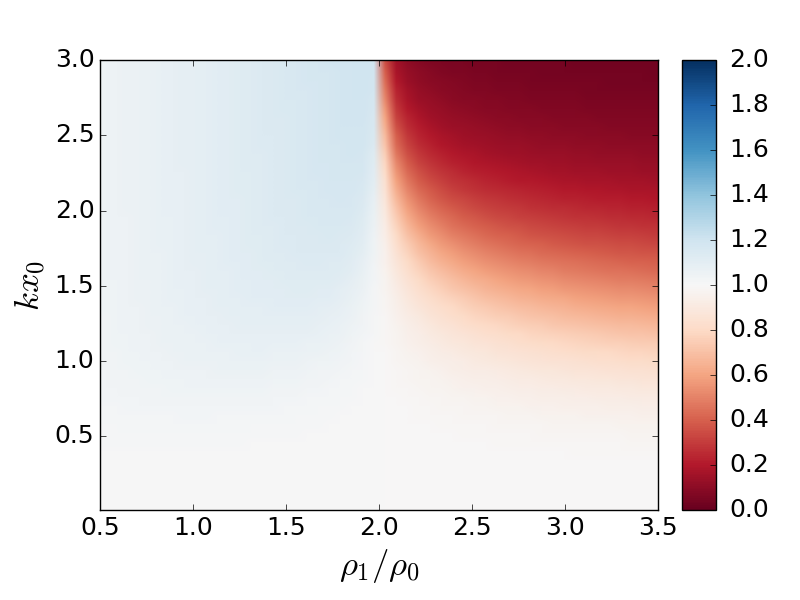
\includegraphics[scale=0.35]{media/slow-kink-surf_amp-ratio.png}
\label{fig: AR slow kink surf}}
\subfloat[Quasi-sausage]{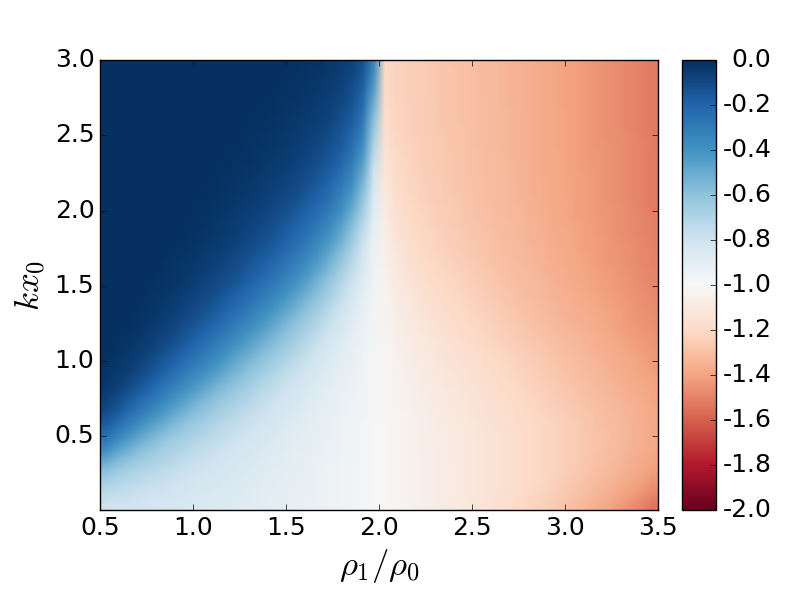
\includegraphics[scale=0.35]{media/slow-saus-surf_amp-ratio.png}
\label{fig: AR slow saus surf}}
\\
\subfloat[Quasi-kink]{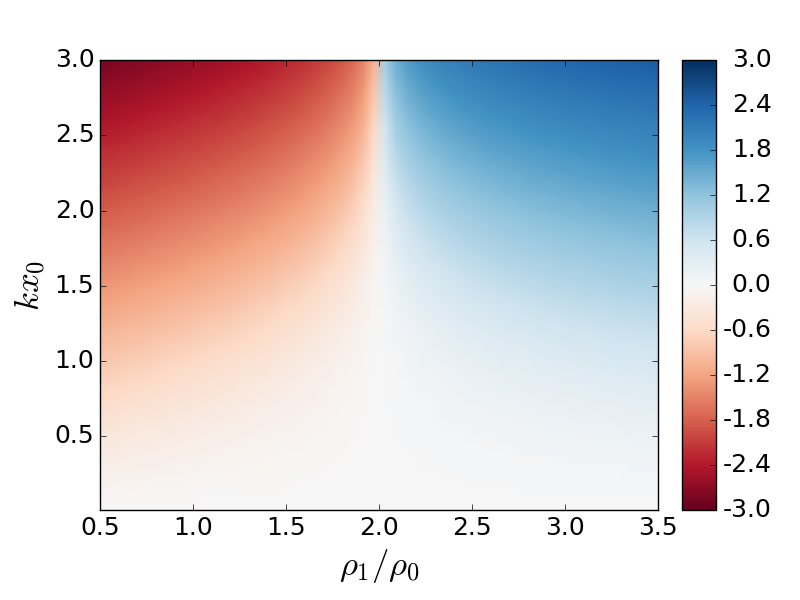
\includegraphics[scale=0.35]{media/slow-kink-surf_min-pert-shift.png}
\label{fig: MPS slow kink surf}}
\subfloat[Quasi-sausage]{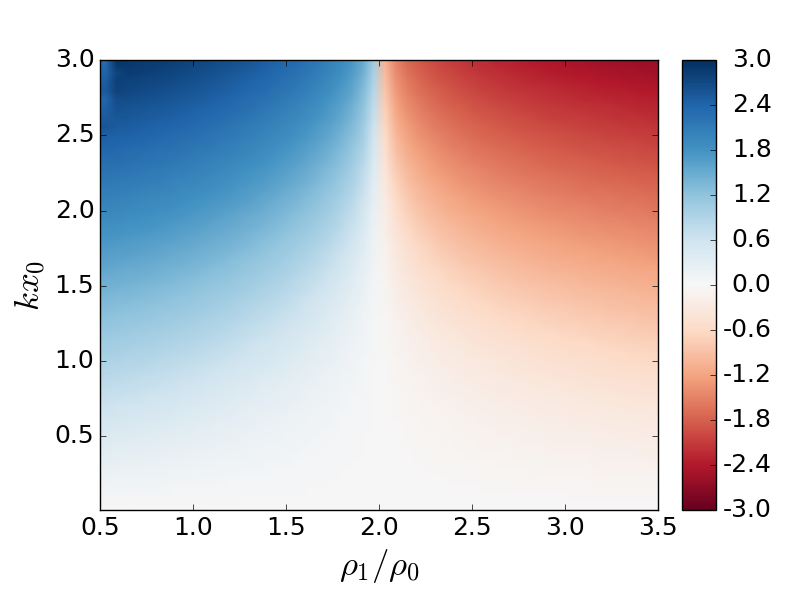
\includegraphics[scale=0.35]{media/slow-saus-surf_min-pert-shift.png}
\label{fig: MPS slow saus surf}}
\caption{The amplitude ratio (\protect\subref*{fig: AR slow kink surf}, \protect\subref*{fig: AR slow saus surf}) and minimum perturbation shift (\protect\subref*{fig: MPS slow kink surf}, \protect\subref*{fig: MPS slow saus surf}) as a function of the slab width, non-dimensionalised as $kx_0$, and the density ratio, $\rho_1/\rho_0$ for slow quasi-kink (\protect\subref*{fig: AR slow kink surf}, \protect\subref*{fig: MPS slow kink surf}) and quasi-sausage (\protect\subref*{fig: AR slow saus surf}, \protect\subref*{fig: MPS slow saus surf}) surface modes. The other density ratio is set to $\rho_2/\rho_0 = 2$ and the characteristic speed ordering inside the slab is $v_\textrm{A}=1.3c_0$ and the sound speed outside the slab is determined to ensure equilibrium pressure balance.}
\label{fig: AR MPS}
\end{figure}

Figure~\ref{fig: AR MPS} illustrate the dependency of the amplitude ratio and minimum perturbation shift on the (non-dimensionalised) slab width, $kx_0$, and the density ratio, $\rho_1/\rho_0$, of one external plasma density to the slab density, holding the other external density fixed. The amplitude ratio is positive (negative) for quasi-kink (quasi-sausage) modes, because the oscillations on each boundary are in phase (anti-phase). Figures~\ref{fig: AR slow kink surf} and~\ref{fig: AR slow saus surf} further shows that, for a given background paramter regime, the boundary with the highest amplitude is different for quasi-kink and quasi-sausage modes. This is demonstrated by the value of the absolute value of the amplitude ratio being greater than 1 for quasi-sausage modes when it is less than 1 for quasi-kink modes, and \textit{vice versa}. This is in agreement with the properties of the eigenmodes of the analogous spring-mass system introduced by \cite{all_etal17}. Figures~\ref{fig: MPS slow kink surf} and~\ref{fig: MPS slow saus surf} demonstrate that the minimum perturbation shift for quasi-kink modes is in the opposite direction to that of quasi-sausage modes, for a given background parameter regime.

The amplitude ratio has a strong (logarithmic) sensitivity to the changes in the external densities, and therefore the external asymmetry, whereas the minimum perturbation shift has only a linear dependency. This means that the amplitude ratio is likely to be a more effective parameter for diagnosing background parameters. Furthermore, observations of the location of the minimum wave power within a solar magnetic slab will be fraught with noise potentially causing the detection of a false minimum. Noise in amplitude ratio measurements is less likely to introduce large errors because we can determine the position of the boundaries of the slab as the location of steep gradients in the wavelength of the observed light, for example.

There are a number of ways that the amplitude ratio and minimum perturbation shift can be used for spatial seismology. Firstly, and most simply, given observed values for the wave frequency parameters (frequency or period and wavenumber or wavelength), the background parameters (plasma density inside and in each external side of the slab, which can then be used to determine the sound speeds by assuming equilibrium pressure balance across the slab boundaries), the spatial structure parameters (slab width), and a spatial wave distribution parameter (amplitude ratio or minimum perturbation shift), we can invert the corresponding expression for the spatial wave distribution parameter, Equation~\eqref{cross-slab ratio saus}, \eqref{cross-slab ratio kink}, \eqref{shift min saus}, or~\eqref{shift min kink}, to estimate the Alfv\'{e}n speed, if the wave mode is known.

\begin{figure}
\centering
\subfloat[Quasi-kink]{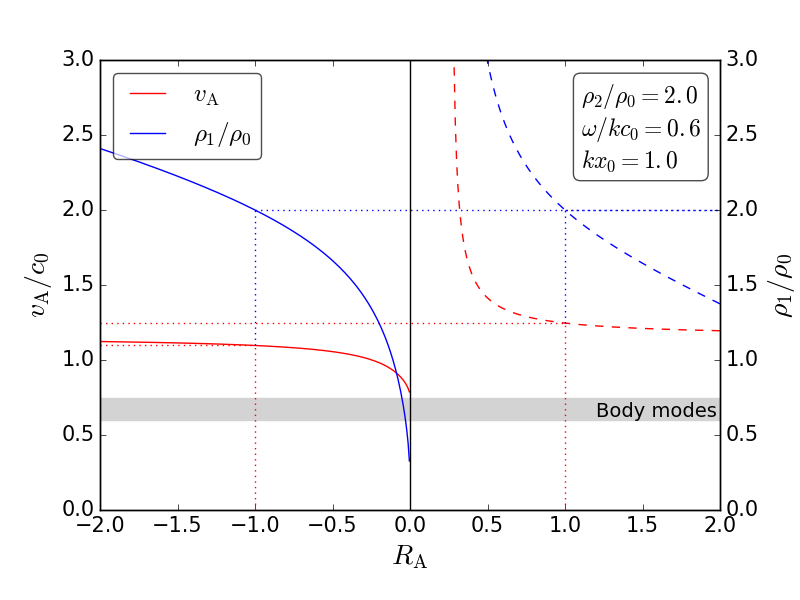
\includegraphics[scale=0.45]{media/RA_vA_approx_2var.png}
\label{fig: RA vA approx}}
\\
\subfloat[Quasi-sausage]{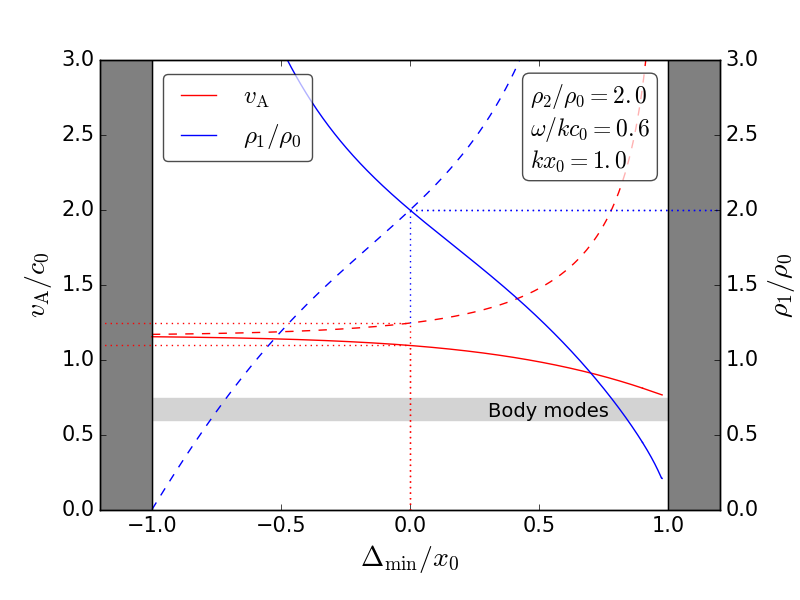
\includegraphics[scale=0.45]{media/DM_vA_approx_2var.png}
\label{fig: DM vA approx}}
\caption{Using prescribed values for the amplitude ratio, $R_\textrm{A}$, \protect\subref{fig: RA vA approx} or minimum perturbation shift, $\Delta_\textrm{min}$, \protect\subref{fig: DM vA approx}, we can use a numerical inversion to approximate background parameters, in this case the Alfv\'{e}n speed, $v_\textrm{A}$, and one of the density ratios, $\rho_1 / \rho_0$. Dashed (solid) lines correspond to the inversion curves for slow quasi-kink (quasi-sausage) surface modes. The dotted lines indicate the inversion for a symmetric slab. The light shaded area indicates the values of the Alfv\'{e}n speed which correspond to body modes, rather than surface modes, so are not important for SMS. The dark shaded region in Figure~\protect\subref{fig: DM vA approx} illustrates that the minimum perturbation shift must be within the slab, that is $|\Delta_\textrm{min} / x_0| < 1$.}
\label{fig: vA approx}
\end{figure}

On a theoretical level, the eigenfunctions of a given system are more sensitive to small changes in the equilibrium parameters than the corresponding eigenfrequencies (Rayleigh-Ritz theorem - references needed, but I cannot find any). This means that spatial seismology techniques will be 


It is more often the case than not all the non-magnetic parameters are well-observable. For example, the density 

The next step along the development of this method is to determine whether magneto-acoustic waves can be set up in an asymmetric waveguide within the characteristic lifetime of such a structure in the solar atmosphere. This can be established analytically (for linear waves with simple initial conditions) and numerically (for nonlinear waves with more sophisticated initial conditions), and will be the subject of future work. Further, a more realistic system, including a magnetic field in the external plasmas, and an equilibrium shear flow, would allow for better application to solar waveguides.



Something about a Bayesian approach for inversion - so that density are not required?



The amplitude ratio has potential as a tool for solar magneto-seismology. The procedure goes as follows:
\begin{itemize}
\item Observe a wave in a slab-like structure,
\item Determine whether the mode is quasi-sausage or quasi-kink,
\item Directly measure the slab width, $x_0$, and the amplitude ratio, $R_\textrm{A}$, using intensity measurements,
\item Estimate the wave period, $2\pi / \omega$, and wavelength, $2\pi / k$,
\item Estimate the density distribution, $\rho_{0,1,2}$, using emission measures, and use these to estimate the sound speeds, $c_{0,1,2}$.
\item Solve \eqref{cross-slab ratio saus} or \eqref{cross-slab ratio kink} for the Alfv\'{e}n speed, $v_\textrm{A}$, numerically or analytically.
\end{itemize}

To solve equation~\eqref{cross-slab ratio saus} or~\eqref{cross-slab ratio kink} directly for $v_\textrm{A}$, a numerical procedure must be followed. The numerical procedure is simple and involves employing a standard root-finding method such as the secant method. To solve analytically, an approximation must be made to simplify Equation~\eqref{cross-slab ratio saus} or~\eqref{cross-slab ratio kink}.

\citep{arr12} for inversion of physical params using MHD seismology.

%%%%%%%%%%%%%%%%%%%%%%%%%%%%%%%%%%%%%%%%%%%%%%%%%%%%%%%%%%%%%%%%%%%%%%%%%%%
%% Appendix
%
%\appendix   

%%%%%%%%%%%%%%%%%%%%%%%%%%%%%%%%%%%%%%%%%%%%%%%%%%%%%%%%%%%%%%%%%%%%%%%%%%%
%% Acknowledgements
%
\begin{acks}
M. Allcock would like to thank the University Prize Scholarship and the SURE Scheme at the University of Sheffield. R. Erd\'{e}lyi acknowledges the support from the UK Science and Technology Facilities Council (STFC), the Royal Society, and is also  grateful to the Chinese Academy of Sciences Presidents International Fellowship Initiative, Grant No. 2016VMA045 for support received. 
\end{acks}

\begin{acks}[Declaration of Potential Conflicts of Interest]
The authors declare that they have no conflicts of interest.
\end{acks}

%%%%%%%%%%%%%%%%%%%%%%%%%%%%%%%%%%%%%%%%%%%%%%%%%%%%%%%%%%%%%%

\bibliographystyle{spr-mp-sola}
\bibliography{Bibliography}

\end{article} 
\end{document}